% !TEX root = 00_MAIN.tex

\chapter{CP-ALS} \label{sec:cpals}

The Canonical Polyadic decomposition (CPD)~\cite{CC70,Harshman70}
is a tensor decomposition that uses an $L^2$ loss function
$f(x,m) \equiv (x-m)^2$ in the optimization in Equation~\ref{eq:gcp}.
CP-ALS --- CP solved via alternating least squares optimization ---
is one approach for performing this tensor decomposition.

\section{Algorithm} \label{sec:cpals_alg}

CP-ALS uses an alternating least squares approach to perform
the optimization. A sketch of the algorithm for three-way tensors 
is included in Algorithm~\ref{alg:cpals}. The method and GentenMPI 
implementation extend to tensors
of any order; for more details, see Kolda and Bader's
survey~\cite{KB09}.  First, factor matrix $A$ is computed with fixed 
factor matrices $B$ and $C$; then $B$ is updated using $A$ and $C$; and
then $C$ is updated using $A$ and $B$.  The algorithm iterates over the 
updates until a desired convergence tolerance is reached or the specified
maximum numer of iterations is exceeded.


\begin{algorithm}
  \caption{CP-ALS algorithm for a three-mode tensor $\X$}
  \label{alg:cpals}
  \begin{algorithmic}[1]
    \Procedure{CP-ALS}{$\X, [\lambda;A,B,C]$}
    \Repeat{}
      \State $A \gets $ MTTKRP($\X,B,C$) $(C^T C * B^T B)^{-1}$
      \State Normalize columns of $A$
      \State $B \gets $ MTTKRP($\X,C,A$) $(A^T A * C^T C)^{-1}$
      \State Normalize columns of $B$
      \State $C \gets $ MTTKRP($\X,A,B$) $(B^T B * A^T A)^{-1}$
      \State Normalize columns of $C$; store norms as $\lambda$
    \Until{converged or max iterations reached}
    \State \Return{$[\lambda;A,B,C]$}
    \EndProcedure
  \end{algorithmic}
\end{algorithm}


\section{Implementation} \label{sec:cpals_impl}

In GentenMPI, CP-ALS is implemented using the MTTKRP algorithm described
in Chapter~\ref{sec:mttkrp}.  The $R \times R$ Gram matrices $(C^T C * B^T B)$
are small enough to replicate on every processor; contributions from each
processor are accumulated using an MPI\_Allreduce operation.  The 
linear systems involving these matrices are solved using LAPACK's GESV method.
Convergence is checked by computing the $L^2$-norm of $\X - \M$.

While GentenMPI's CP-ALS can function with any distribution of the tensor
and factor matrices, faster performance and better scaling is achieved when
the number of tensor entries per processor is balanced and tensor indices
are localized to reduce the number of factor matrix entries needed in MTTKRP.
The SPLATT tensor code provides a ``medium-grain'' decomposition in which
the tensor is divided into subtensors with roughly uniform number of 
nonzeros per subtensor~\cite{SK16}. 
In each mode, then, expand and fold communication is done among 
processors within a slice of subtensors.
A illustration of a medium-grain decomposition is in Figure~\ref{fig:medgrain}.
For a three-way tensor, $P=48$ processors are organized into a three-way 
$6 \times 4 \times 2$ grid.  
Cuts in each mode then greedily assign tensor slices to processors in a way
that balances the number of nonzero entries.

\begin{figure}[ht]
   \centering
   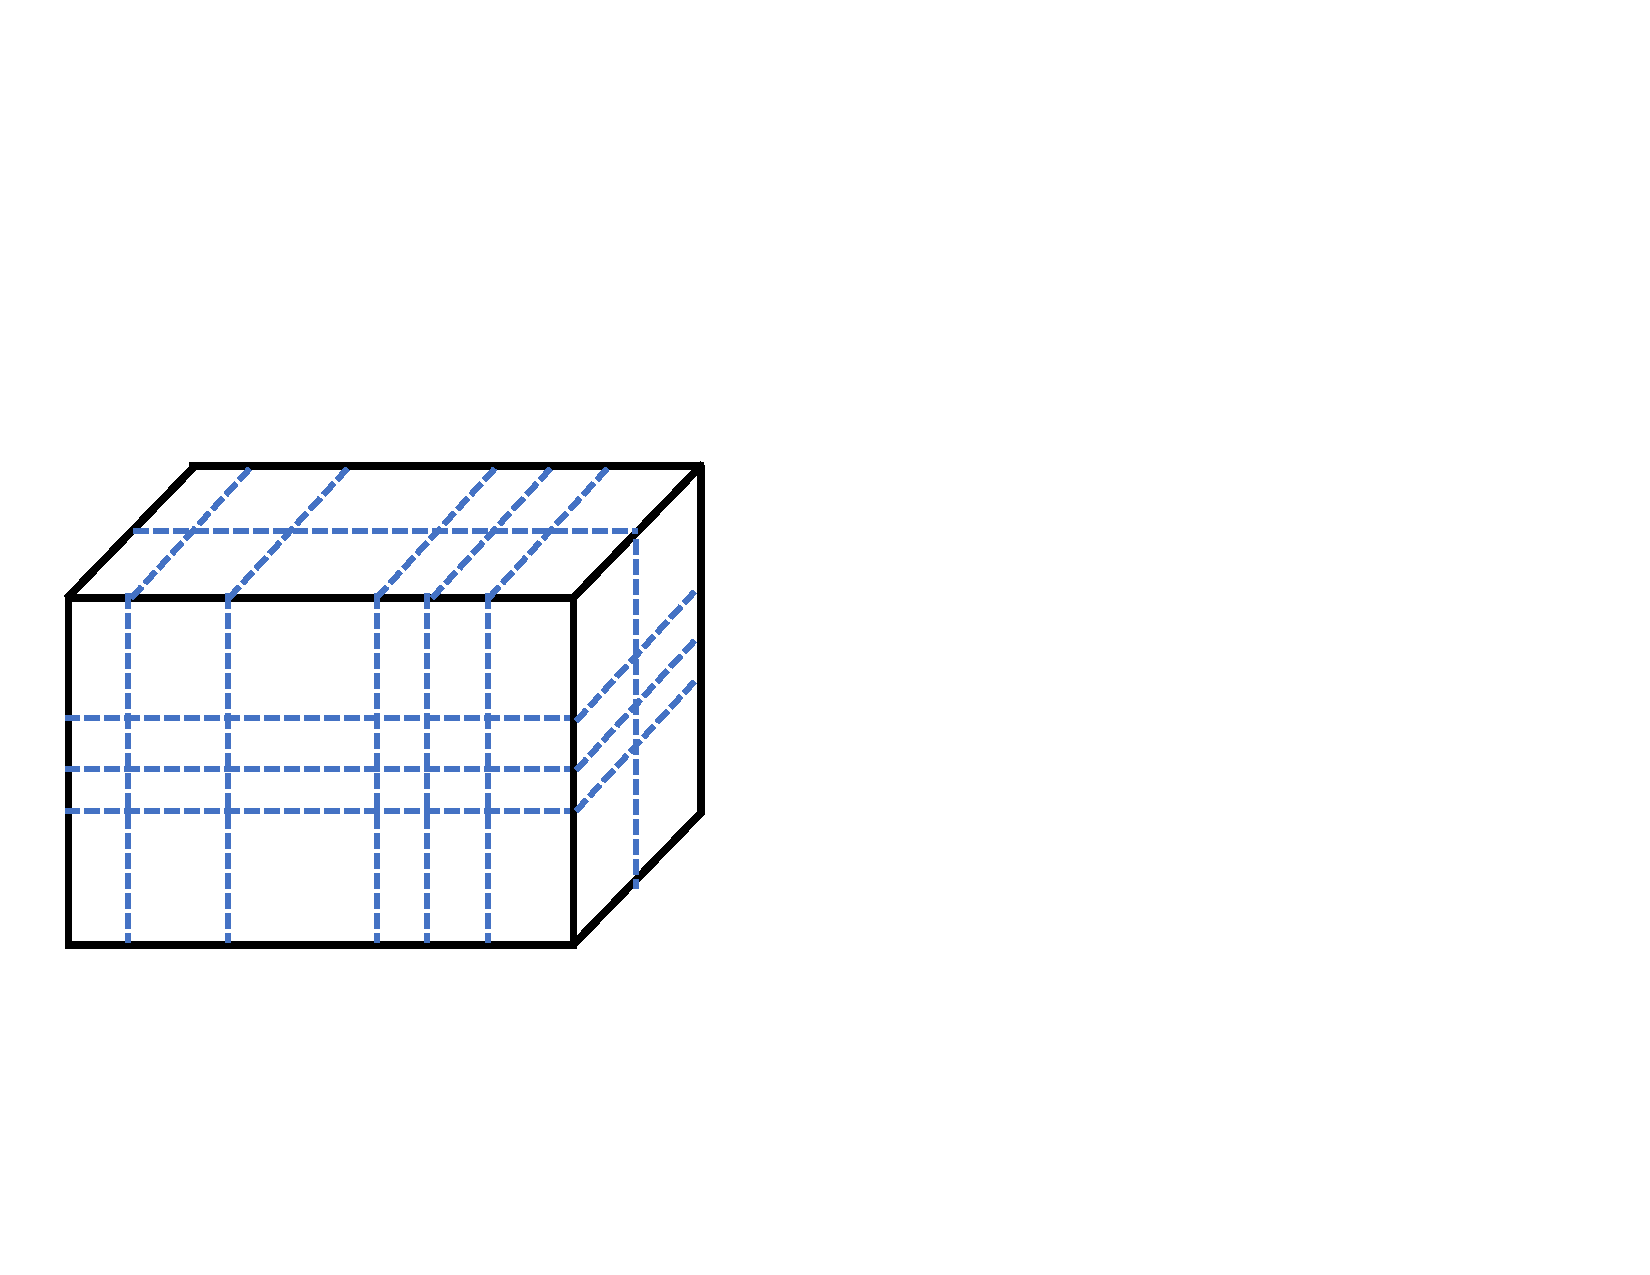
\includegraphics[keepaspectratio=true, width=2.5in]{figs/medgrain}
   \caption[SPLATT medium-grain distribution]{Illustration of a 
 SPLATT medium-grain distribution~\cite{SK16}
 of a three-way tensor to 48 processors}
   \label{fig:medgrain}
\end{figure}

We adopt this medium-grain decomposition for CP-ALS in GentenMPI. Because equal
number of nonzers are assigned to each processor, this decomposition 
provides good load balance in the MTTKRP computation.  While it doesn't 
explicitly attempt to minimize communication during MTTKRP, it provides 
reasonable alignment between factor matrix distributions and needed tensor 
entries.  And it is inexpensive to compute compared to partitions that 
do explicitly attempt to reduce communication, such as the hypergraph methods
of Kaya and Ucar~\cite{KayaUcarSC15}.

We use
the default Trilinos {\tt Map} layout (Section~\ref{sec:maps})
for factor matrices; that is, on $P$ processors,
factor matrix $A \in \mathbb{R}^{I \times R}$ is divided into $P$ chunks
of length $I/P$, with processor 0 receiving chunk \{$1,2,\ldots,I/P$\},
processor 1 receiving chunk \{$I/P+1,\ldots,2I/P$\}, and so on.


\section{Experimental Results} \label{sec:cpals_exp}

The main motivation in creating GentenMPI is to enable decomposition of
tensors too large to fit into a single node's memory.  To demonstrate this
capability, we study the weak-scaling of GentenMPI's CP-ALS by 
generating random sparse tensors and apply CP-ALS to them.  The generated
tensors are four-way tensors with 64 million nonzeros per processor and the 
mode lengths adjusted to maintain constant nonzero density of 0.001024.
With these characteristics, the tensor size is 12.6 Terabytes on 8192
processors:  524 billion nonzeros with four integers and one double per nonzero.

Weak scaling results on Sandia's SkyBridge cluster (2.6 GHz Intel Sandy
Bridge nodes with Infiniband network) are shown in Figure~\ref{fig:huge}.
We show both the average time per CP-ALS iteration and MTTKRP within a 
CP-ALS iteration.  Clearly, the MTTKRP kernel dominates the CP-ALS computation.
Weak scaling is very good, but degrades slightly due to an increased number
of neighboring processors (and, thus, of messages) as the number of 
processors increases. (Envision more layers of processors being added to
the processor distribution in Figure~\ref{fig:medgrain} as the number of 
processors increases.)


\begin{figure}[ht]
   \centering
   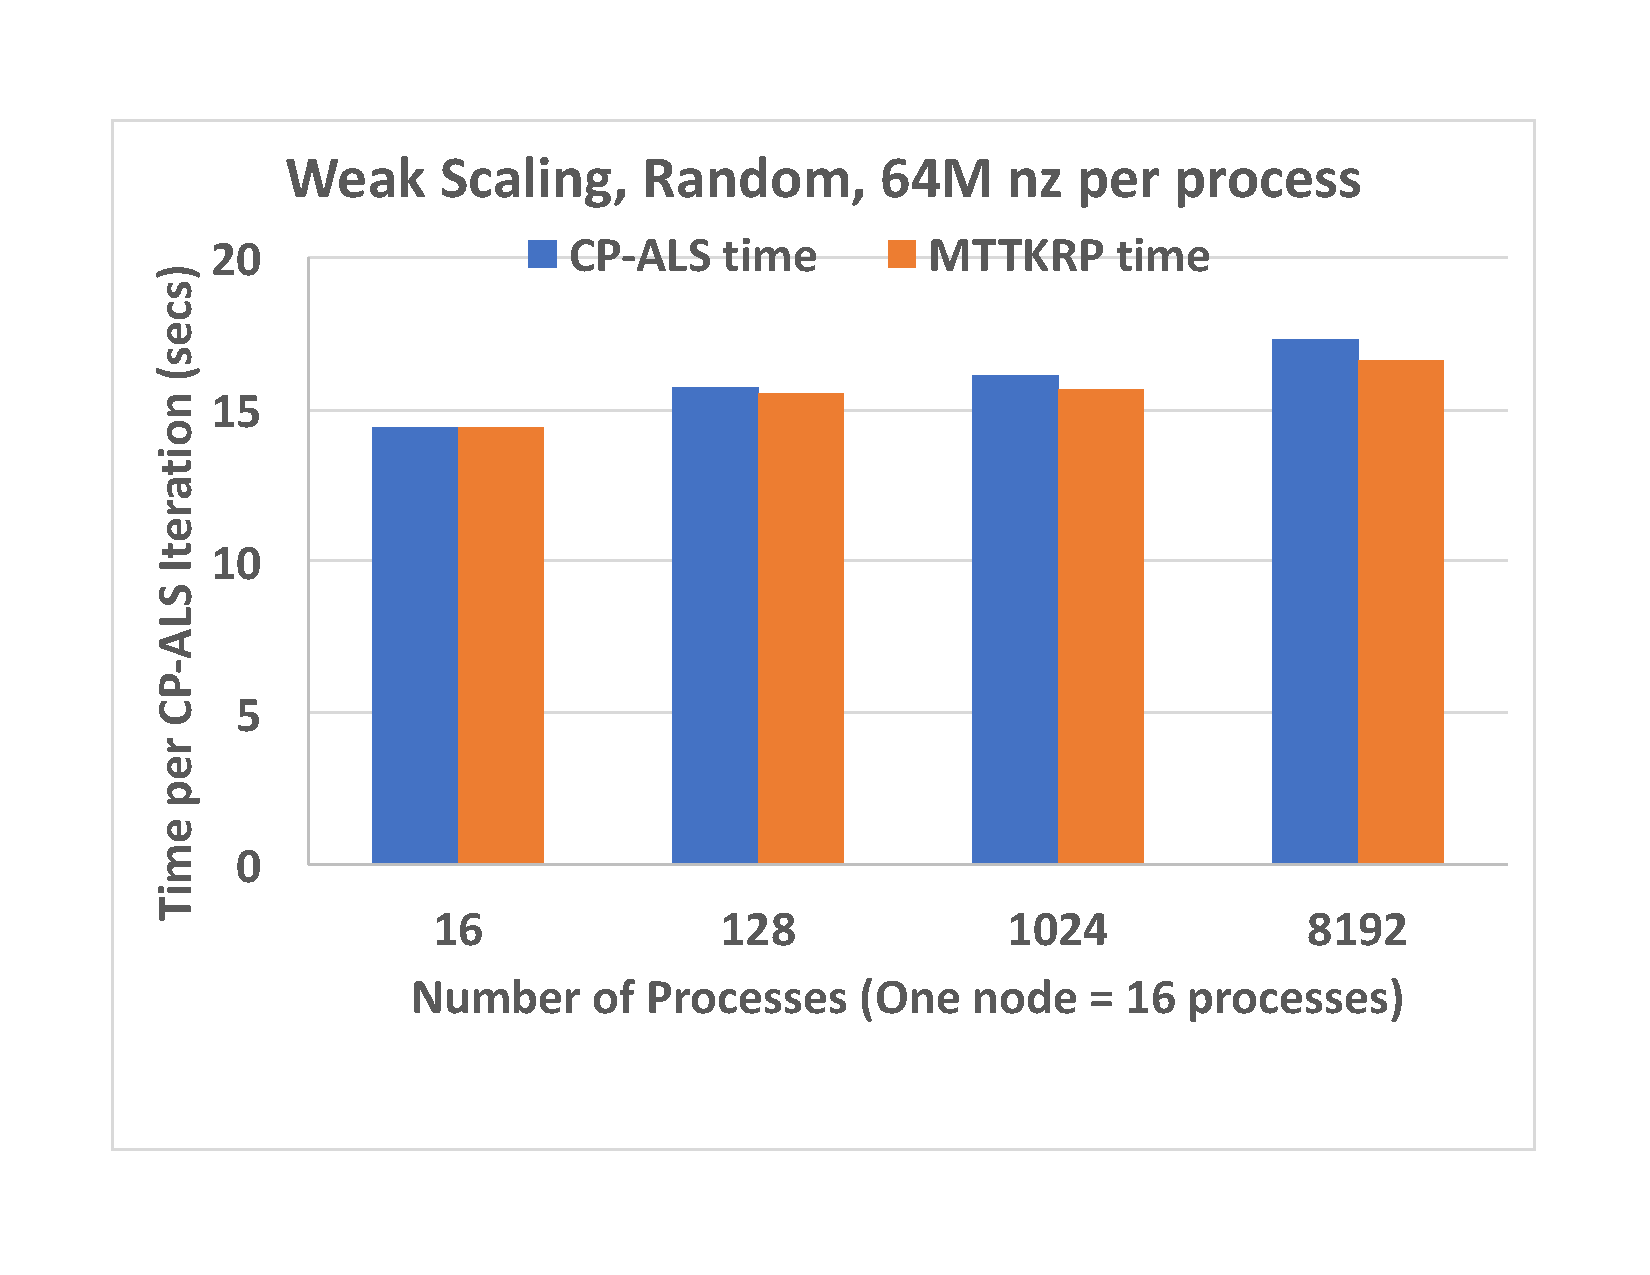
\includegraphics[keepaspectratio=true, width=4.5in]{figs/huge}
   \caption[Weak scaling of CP-ALS]{Weak scaling of CP-ALS on a four-way random tensor:  the time for one CP-ALS iteration is in blue, with the MTTKRP time per iteration in orange.
The largest tensor, decomposed on 8192 processors, is 12.6 Terabytes.}
   \label{fig:huge}
\end{figure}



We next examine the strong scaling of GentenMPI's CP-ALS implementation,
comparing GentenMPI's performance with SPLATT~\cite{SK16} and 
Genten~\cite{PK19}.
SPLATT can run with distributed memory parallelism only (``MPI-only'') or
with hybrid distributed memory and shared memory threading (``MPI+OpenMP'').
We compare with both configurations.  
For the MPI-only case, we use the same number of 
MPI ranks for SPLATT and GentenMPI.  For MPI+OpenMP, we use 16 threads per 
MPI rank and one MPI rank in SPLATT for every 16 MPI ranks in GentenMPI.
For 16 processor runs, we compare with Genten with 16 threads.

We begin with the \emph{delicious-4d} tensor from the FROSTT~\cite{FROSTT} 
tensor collection,
a $532,924 \times 17,262,471 \times 2,480,308 \times 1443$ tensor with 140 million
nonzeros.
We run with 16 to 1024 cores, with rank $R$ ranging from 8 to 128.
Times per CP-ALS iteration are shown in Figure~\ref{fig:cpals_delicious}.
We see that the strong scaling of GentenMPI is good in all experiments.
Runtimes are generally faster than SPLATT MPI-only; multithreading does
make SPLATT's performance with MPI+OpenMP superior to GentenMPI.
GentenMPI's runtimes are acceptable when compared to Genten.  GentenMPI
has the benefit that it can access sufficient memory for the $R=128$ case,
while Genten has the advantage that it can run on both multithreaded CPUs and 
GPUs.

\begin{figure}[ht]
   \centering
   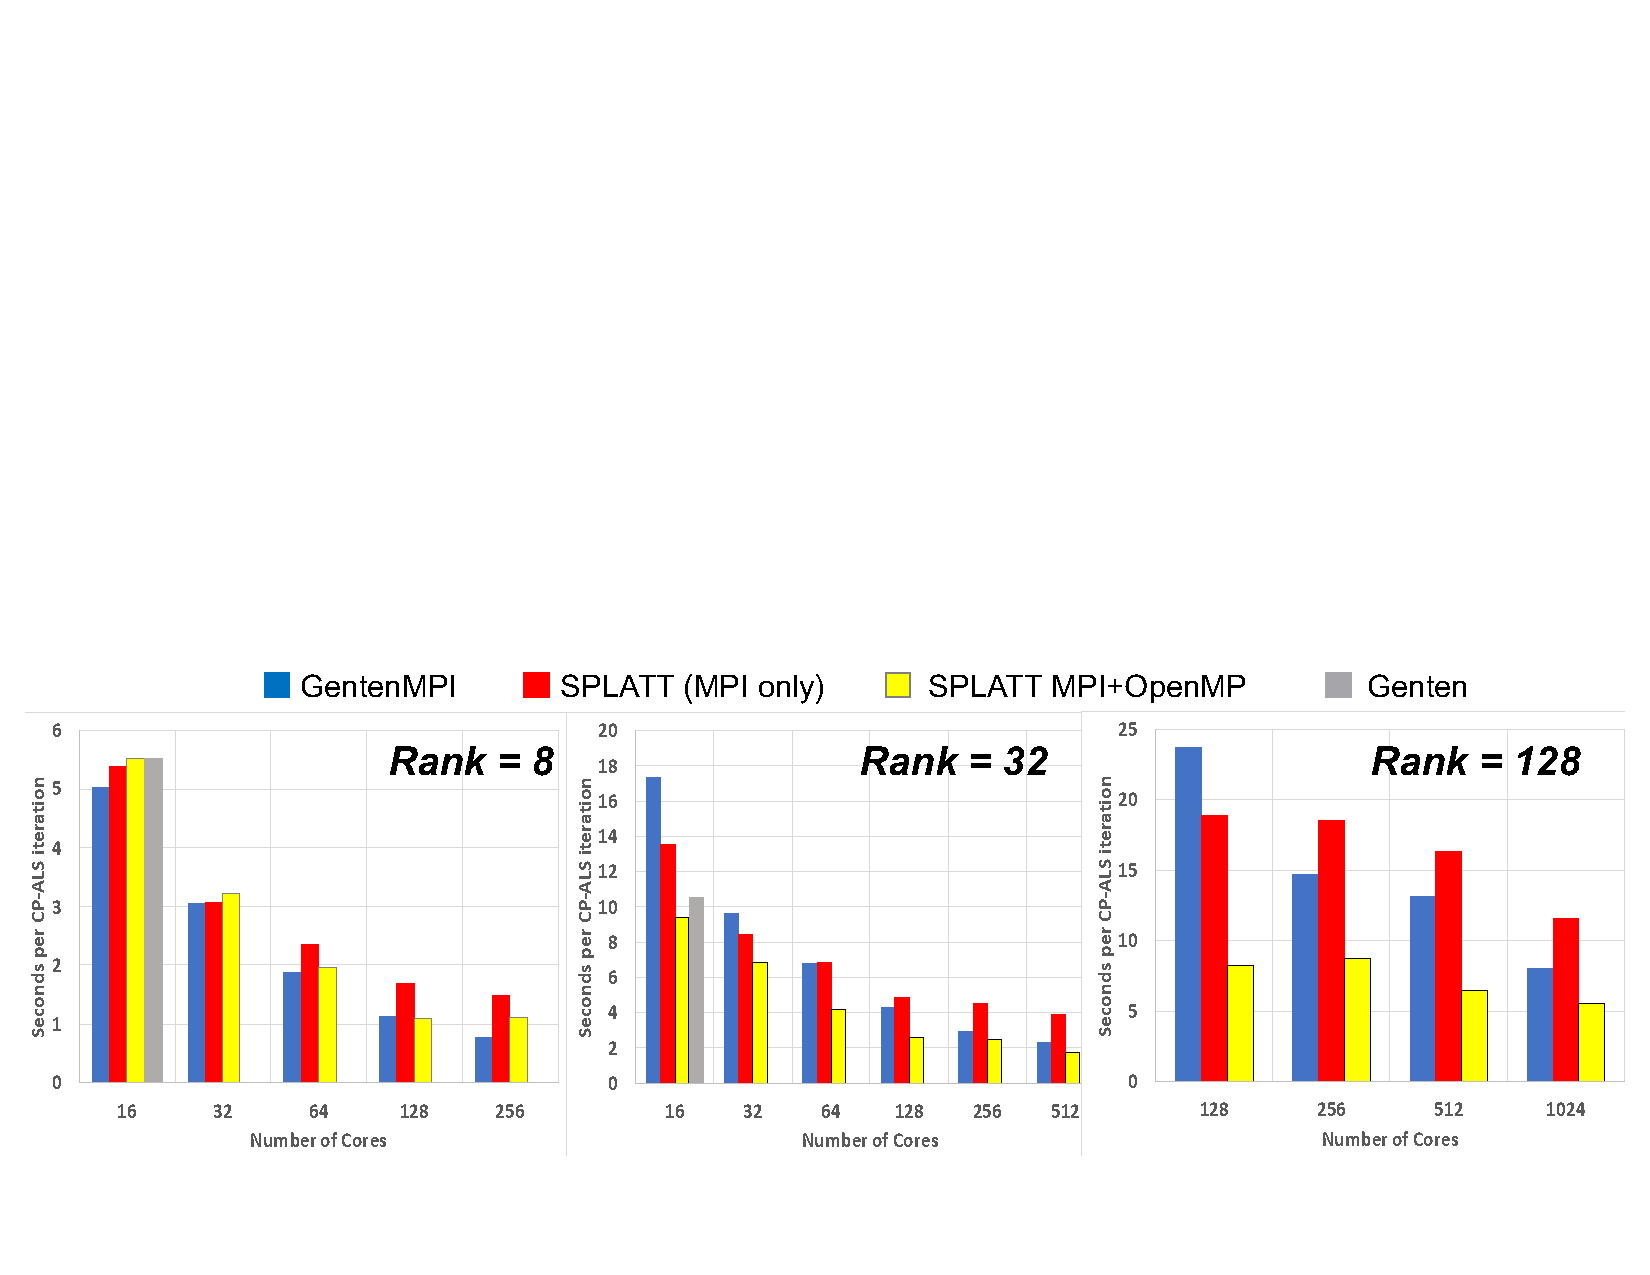
\includegraphics[keepaspectratio=true, width=6in]{figs/cpals_delicious}
   \caption[Strong scaling of CP-ALS on \emph{delicious-4d} tensor]{Strong scaling of CP-ALS on the \emph{delicious-4d} tensor from the FROSTT~\cite{FROSTT} collection.  GentenMPI times per CP-ALS iteration are compared
with those from Genten~\cite{PK19} and SPLATT~\cite{SK16} with MPI-only and MPI+OpenMP.}
   \label{fig:cpals_delicious}
\end{figure}



We demonstrate GentenMPI on the larger \emph{amazon-reviews} tensor from FROSTT,
a $4.8M \times 1.8M \times 1.8M$ tensor with 1.7 billion nonzeros.  This tensor is 
too large to fit in a single node of SkyBridge, so comparisons with Genten
are not possible.  For this tensor, we see in Figure~\ref{fig:cpals_amazon}
that GentenMPI's implementation is
faster than both SPLATT MPI-only and SPLATT MPI+OpenMP.  Strong scaling is 
good out to 1024 cores.

\begin{figure}[ht]
   \centering
   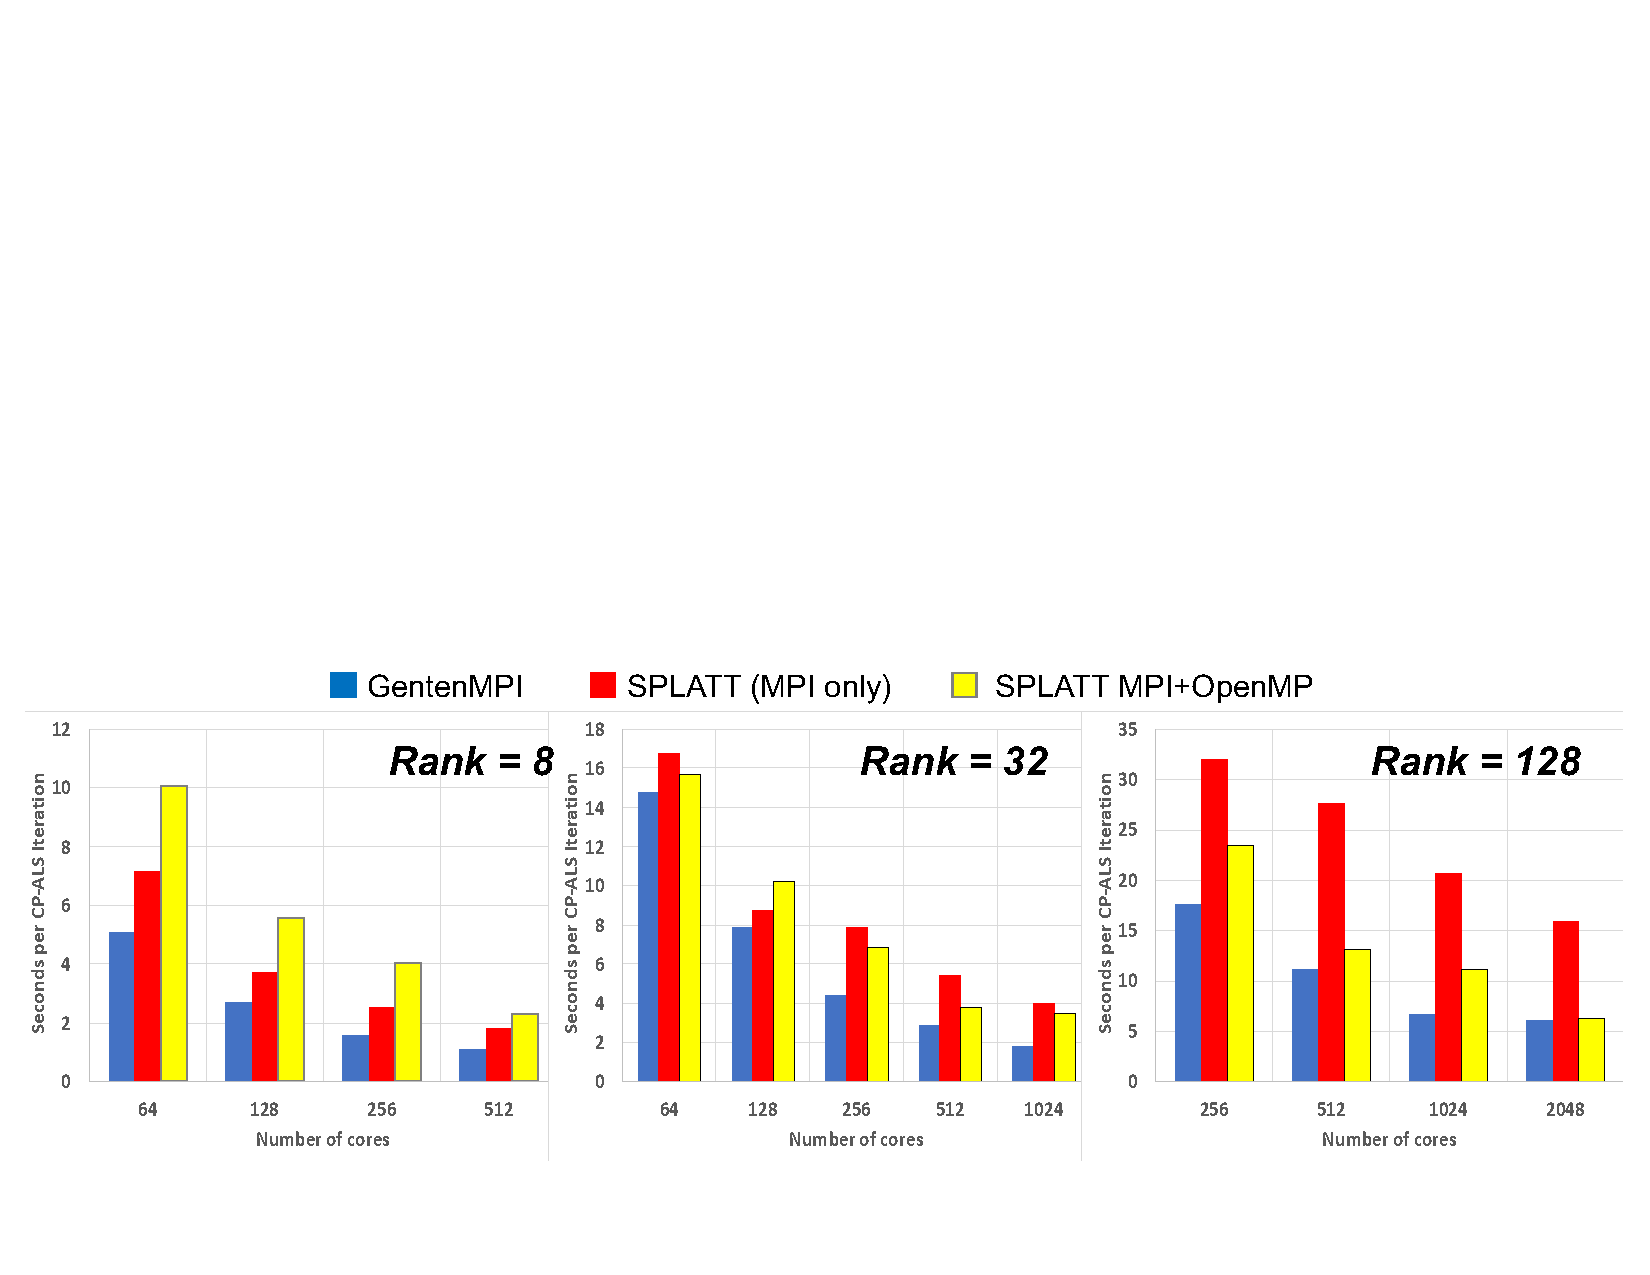
\includegraphics[keepaspectratio=true, width=6in]{figs/cpals_amazon}
   \caption[Strong scaling of CP-ALS on \emph{amazon-reviews} tensor]{Strong scaling of CP-ALS on the \emph{amazon-reviews} tensor from the FROSTT~\cite{FROSTT} collection.  GentenMPI times per CP-ALS iteration are compared
with those from SPLATT~\cite{SK16} with MPI-only and MPI+OpenMP.}
   \label{fig:cpals_amazon}
\end{figure}


